\documentclass[12pt,norsk,a4paper]{article}
\usepackage[norsk]{babel}
\usepackage[norsk]{isodate}
\usepackage[T1]{fontenc}
\usepackage{parskip}
\usepackage{url}
\usepackage{listings}
\author{fridatbe}
\title{IN1080 --- Obligatorisk oppgave 2}
\date{\today}
\usepackage[small,euler-digits]{eulervm}
\usepackage{color}
% \usepackage{minted}
\usepackage{xcolor}
\definecolor{LightGray}{gray}{0.9}
\usepackage{a4wide}
\usepackage[top=2cm]{geometry}
\usepackage{graphicx}
\graphicspath{ {./fig/} }
\newcommand{\tuple}[1]{\ensuremath{\langle #1\rangle}}
\newcommand{\set}[1]{\ensuremath{\{#1\}}}
\newcommand{\imp}{\ensuremath{\rightarrow}}
\newcommand{\M}{\ensuremath{\mathcal{M}}}
\newcommand{\AF}{edge from parent[draw=none]}
\newcommand{\NODE}[1]{\{node \{\ensuremath{#1}\}\}}
\usepackage[explicit]{titlesec}
\titleformat{\section}{\normalfont\Large\bfseries}{}{0em}{#1\ \thesection}


\begin{document}
    \maketitle
    \renewcommand{\thesubsection}{(\alph{subsection})}
    \newpage

    \section{Oppgave}
        Figur:\\
        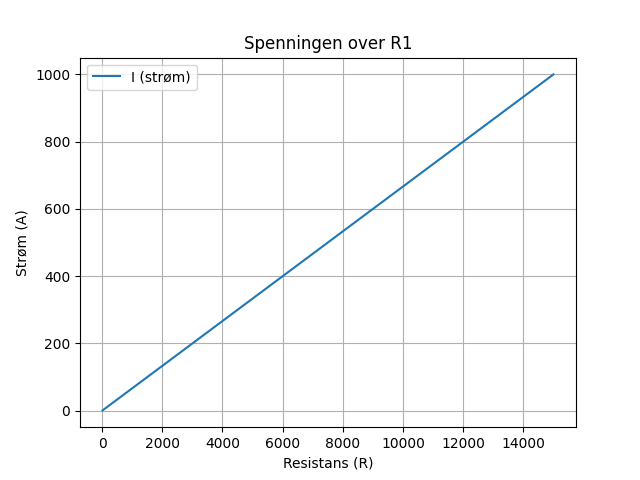
\includegraphics[width=1\textwidth]{funksjon.png}\\
        Kode:\\
        \begin{lstlisting}[language=Python]
            from matplotlib import pyplot as plt
            import numpy as np

            V = np.arange(1, 10, 0.1)
            plt.xticks(np.arange(min(V), max(V)+1, 1))
            I = V/100
            plt.title("Strømmen ved 100 Ohm resistans")
            plt.xlabel("Spenning(V)")
            plt.ylabel("Strøm (A)")
            plt.plot(V,I, label='I (strøm)')
            plt.legend()
            plt.grid()
            plt.savefig("opg1.png");
        \end{lstlisting}
    \newpage

    \section{Oppgave}
        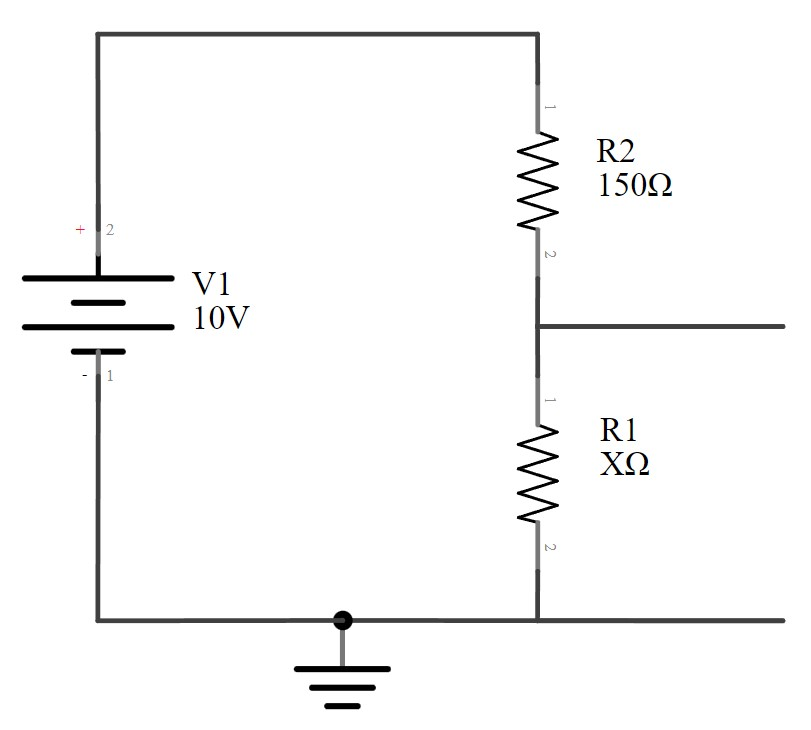
\includegraphics[width=0.5\textwidth]{figur.jpg}\\
        Får oppgitt: \\
        $ V_1 = 10V, V_x = 2.5V, R_2 = 150 Ohm$ \\\\
        Formel for spenningen i en gitt node:\\
        $V_x=V_1 * \frac{R_1}{R_1 + R_2}$ \\\\
        Fyller inn tallene i formelen:\\
        $2.5V = 10V * \frac{R_1}{R_1 + 150 Ohm}$\\\\
        % Løser for R_1 og finner at: \\
        $R_1 = 50 Ohm$\\\\
        Fordi:\\
        $2.5V = 10V * \frac{50 Ohm}{50 Ohm + 150 Ohm}$\\\\
        $2.5V = \frac{500 (V*Ohm)}{200 Ohm}$\\
    \newpage

    \section{Oppgave}
        Figur:\\
        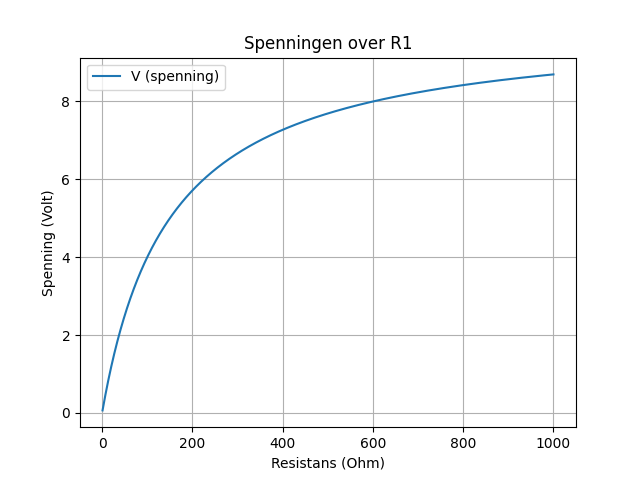
\includegraphics[width=1\textwidth]{opg2.png}\\
        Kode:\\
        \begin{lstlisting}[language=Python]
            from matplotlib import pyplot as plt
            import numpy as np
            R = np.arange(1, 1000, 0.1)
            V = 10*(R/(R+150))
            plt.title("Spenningen over R1")
            plt.xlabel("Resistans (Ohm)")
            plt.ylabel("Spenning (Volt)")
            plt.plot(R, V, label='V (spenning)')
            plt.legend()
            plt.grid()
            plt.savefig("opg2.png");
        \end{lstlisting}
        
    \newpage


    \section{Oppgave}
    Jeg fant ikke en resistor på 10 kOhm i Arduinosettet, så erstattet R2 med en resistor på 16 kOhm\\
    Får derfor oppgitt: \\
    $V_s = 5V, R_1 = 4.7 kOhm, R_2 = 16 kOhm$ \\\\
    Formel for spenningen i en gitt node:\\
    $V_x = V_1 * \frac{R_1}{R_1 + R_2}$ \\\\
    Fyller inn tallene i formelen:\\
    $V_x = 5 V * \frac{4.7 kOhm}{4.7 kOhm + 16 kOhm}$\\\\
    $V_x =  1.1V$\\\\

    Måling av spenning:\\
    $V_x =  1.6V$\\

    Mulige årsaker til avvik:
    \begin{itemize}
        \item Mulitmeteret/voltmeteret er unøyaktig
        \item Multimeteret påvirker spenningen ved at den leder strøm
        \item Resistorene, lederne og spenningskilden er funksjonelle og ikke optimale, 
        dvs. elementene ikke gir konstant påvirkning til kretsen (eks. resistorene gir lavere motstand ved høyere spenning)
    \end{itemize}
    \newpage

    \section{Oppgave}
        Her er spenningsdeleren med LED koblet i parallell med potentiometeret, da vediene gikk fra 0 til 536 vred jeg på potentiometeret og LED-lyset skrudde seg av og på, tilsvarende\\
        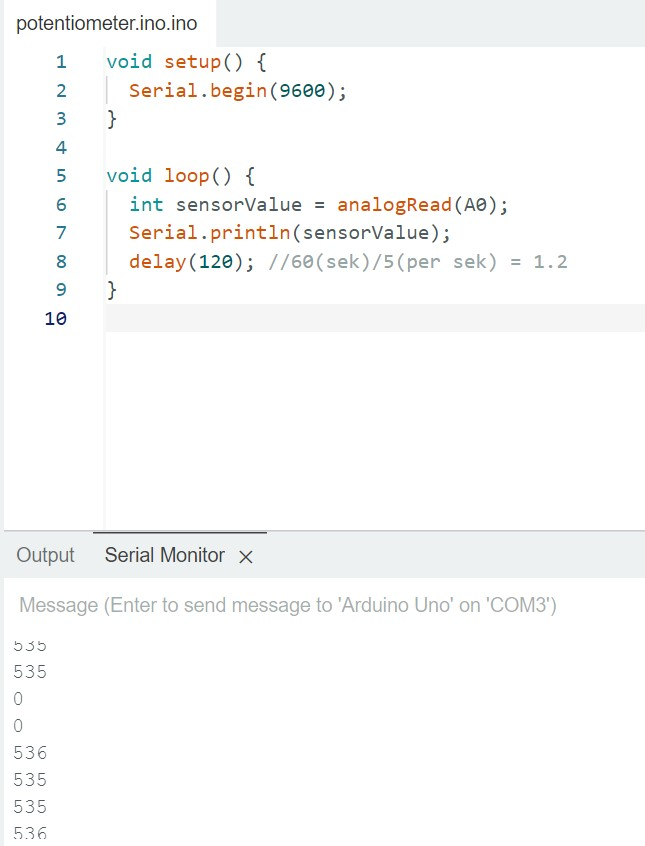
\includegraphics[width=0.5\textwidth]{medLED.jpg}\\
    \newpage

    \section{Oppgave}
        Observerte at verdiene på spenningen ble mye lavere (ned til 0) da jeg la på last (første strømmen gjennom fingrene mine)\\
        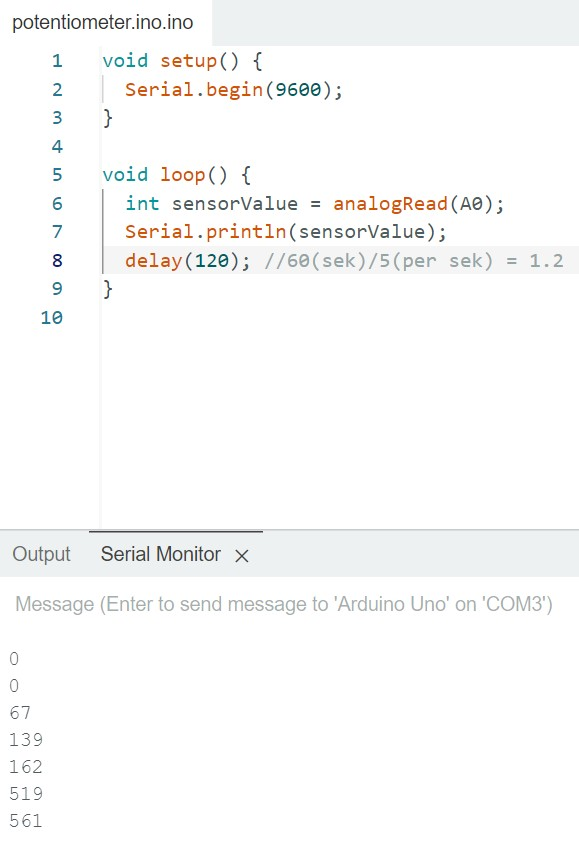
\includegraphics[width=0.5\textwidth]{medLast.jpg}\\
    \newpage



\end{document}
